\chapter{Prezentacja systemu}

\section{Urządzenie pomiarowe}
Na Rys. \ref{prototyp} przedstawiono prototyp urządzenia pomiarowego z sensorem
temperatury DS18B20 oraz sensorem DHT11 służącym do wykonywania pomiarów wilgotności oraz temperatury powietrza. 
DS18B20 to prosty sensor temperatury wykorzystujący jeden
pin jako linię danych. Każda sztuka posiada unikalny 64 bitowy adres, który
umożliwia wykorzystanie wielu takich sensorów na jednej linii danych poprzez
dostęp adresowy. Sensor charakteryzuje się pracą w zakresie od -55 do 125 stopni 
Celsjusza z typowym błędem +-0.5 stopnia w zakresie od -10 do 85 stopni Celsjusza.
DHT11 charakteryzuje się pracą w zakresie od 20\% do 90\% wilgotności powietrza z
typowym błędem +- 4\%. Umożliwia również na pomiar temperatur w zakresie od 0 do 50
stopni Celsjusza z typowym błędem wynoszącym 2 stopnie Celsjusza.
\begin{figure}[h!]
  \centering
  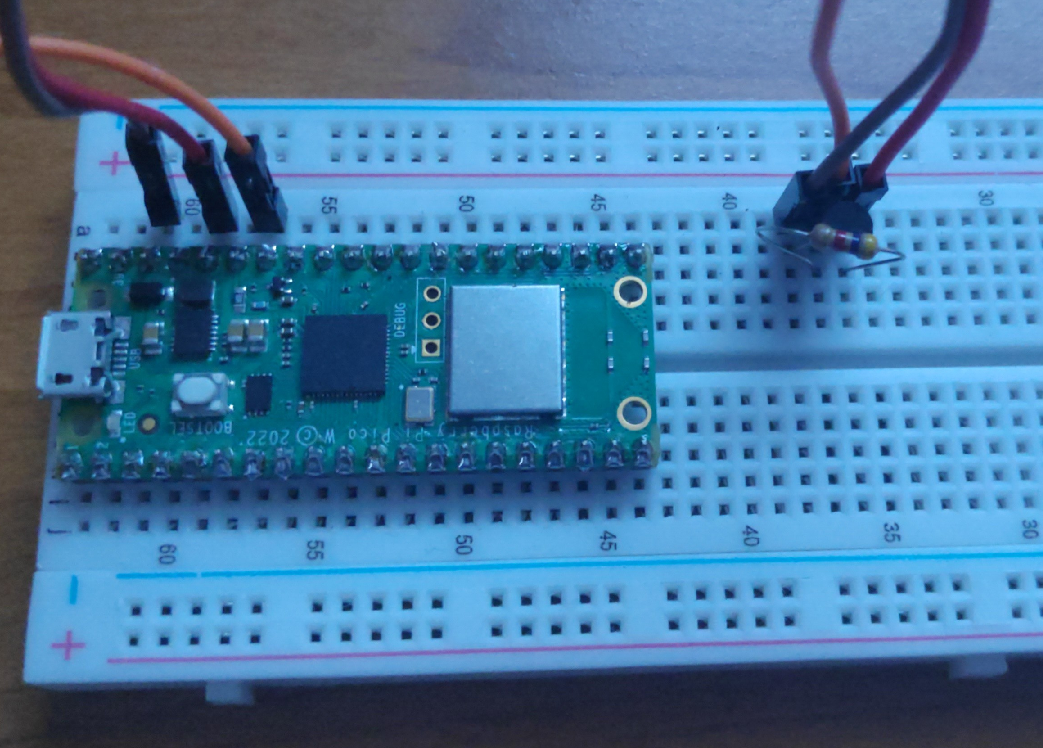
\includegraphics[width=\textwidth]{prototyp}
  \caption{Prototyp urządzenia pomiarowego}
  \label{prototyp}
\end{figure}

\section{Aplikacja kliencka}
Pierwszym krokiem, który wykonuje użytkownik po uruchomieniu aplikacji jest 
proces logowania. Aby zwiększyć bezpieczeństwo danych wszystkie funkcjonalności
dostępne są jedynie aktywnym kontom użytkowników.
Interfejs logowania przedstawiono na Rys. \ref{atmosphere:signin}.
\begin{figure}[h!]
  \centering
  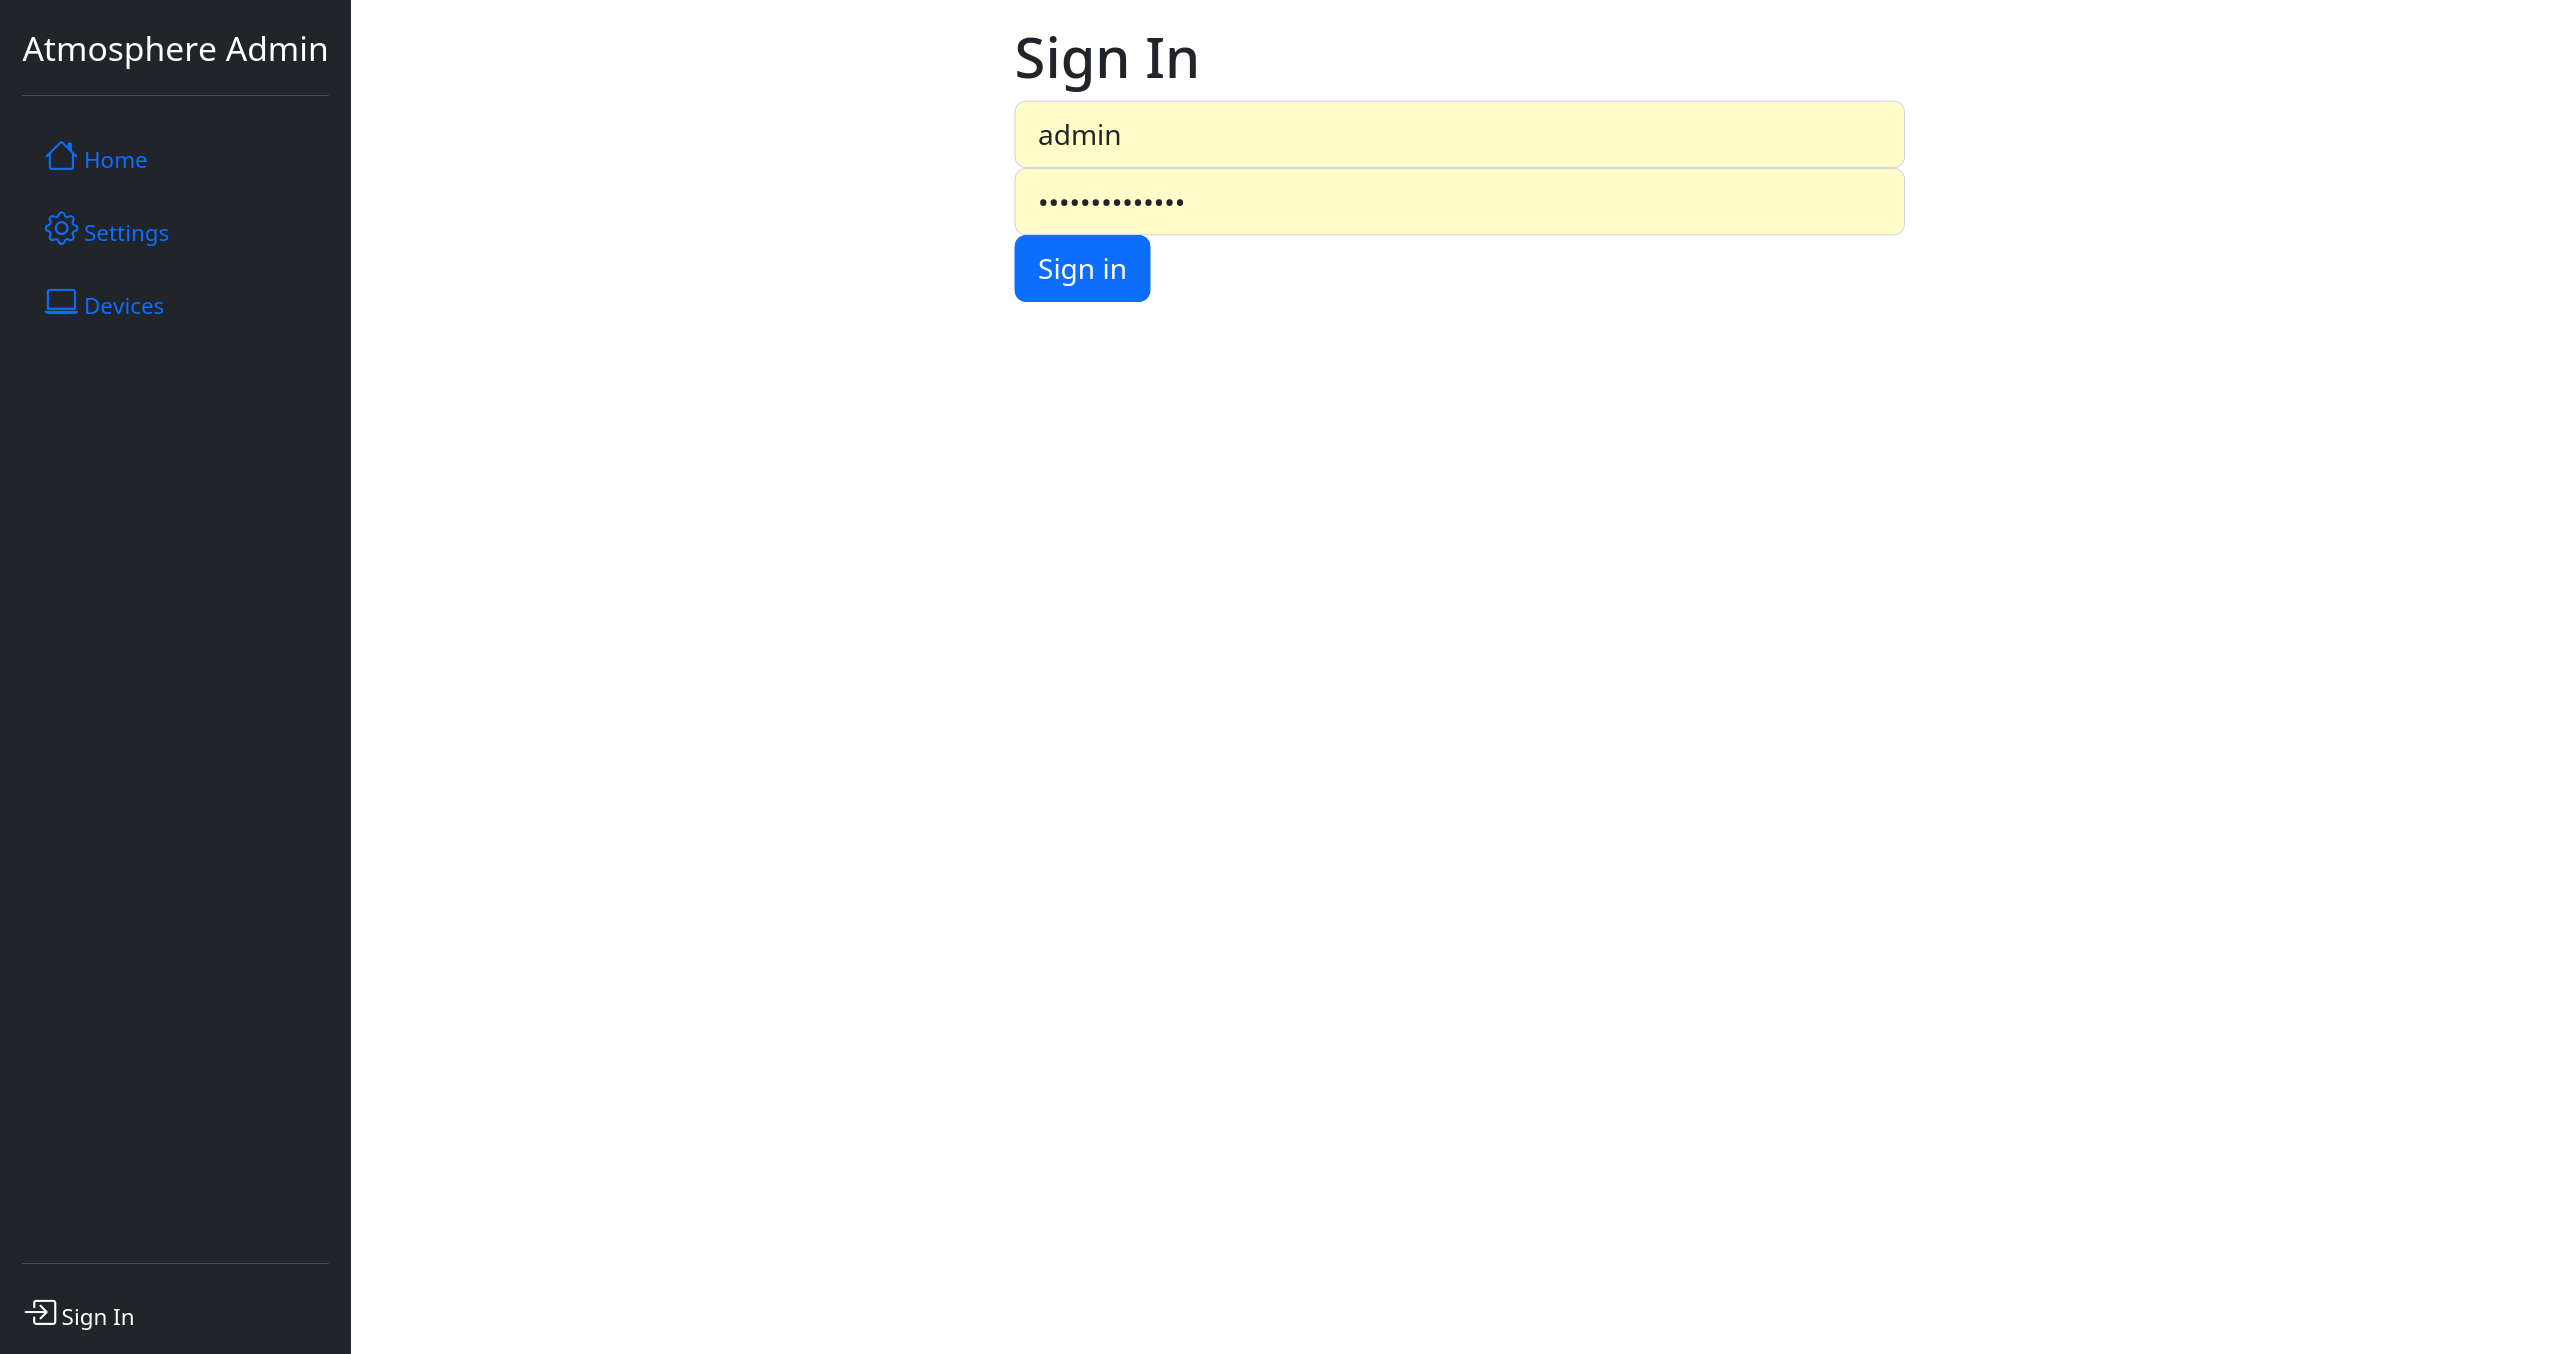
\includegraphics[width=\textwidth]{signin}
  \caption{Widok logowania}
  \label{atmosphere:signin}
\end{figure}
W przypadku podania błędnych danych serwer zwraca informację o błędzie, która następnie
wyświetlana jest w formie powiadomienia użytkownikowi. Przykładową zawartość przedstawiono
na Rys. \ref{atmosphere:failedsignin}.
\begin{figure}[h!]
  \centering
  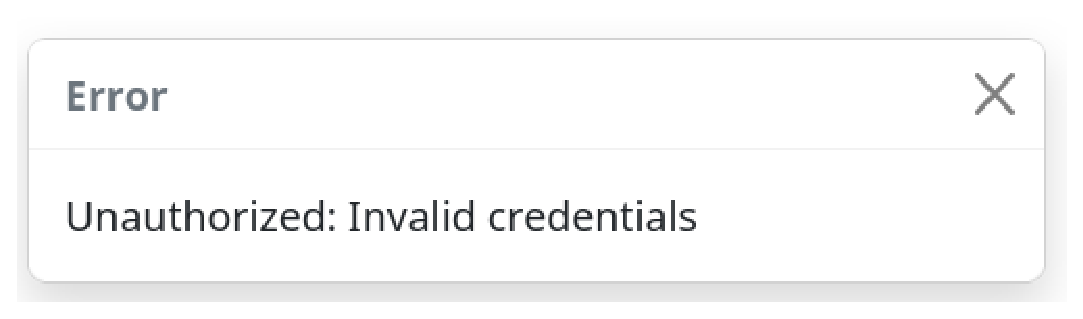
\includegraphics[width=\textwidth]{failedsignin}
  \caption{Informacja o niepoprawnych danych logowania}
  \label{atmosphere:failedsignin}
\end{figure}
Po udanym zalogowaniu w zależności od poziomu uprawnień użytkownik ma dostęp
do pozostałych zasobów aplikacji.
W tym samym momencie aplikacja łączy się z kanałem WebSocket odpowiedzialnym za
wysyłanie powiadomień o niespodziewanych wydarzeniach, tj. przekroczenie
wartości parametrów. Aby je utrzymać aplikacja wysyła wykorzystując te samo
połączenie wiadomość o treści "ping" co 30 sekund. W przypadku, gdy
wystąpi niespodziewane zdarzenie oraz kanał jest aktywny aplikacja otrzymuje
o tym wiadomość z serwera, a następnie wyświetlana jest w formacie powiadomienia
podobnym do wcześniej przedstawionego powiadomienia o nieudanym logowaniu.
Zawartość powiadomienia może zostać dynamicznie zmieniona przez użytkownika
jak i bardziej zaawansowana logika weryfikacji odczytów. Przykładowa konfiguracja
została przedstawiona na Rys. \ref{atmosphere:validation_rule}.
\begin{figure}[h!]
  \centering
  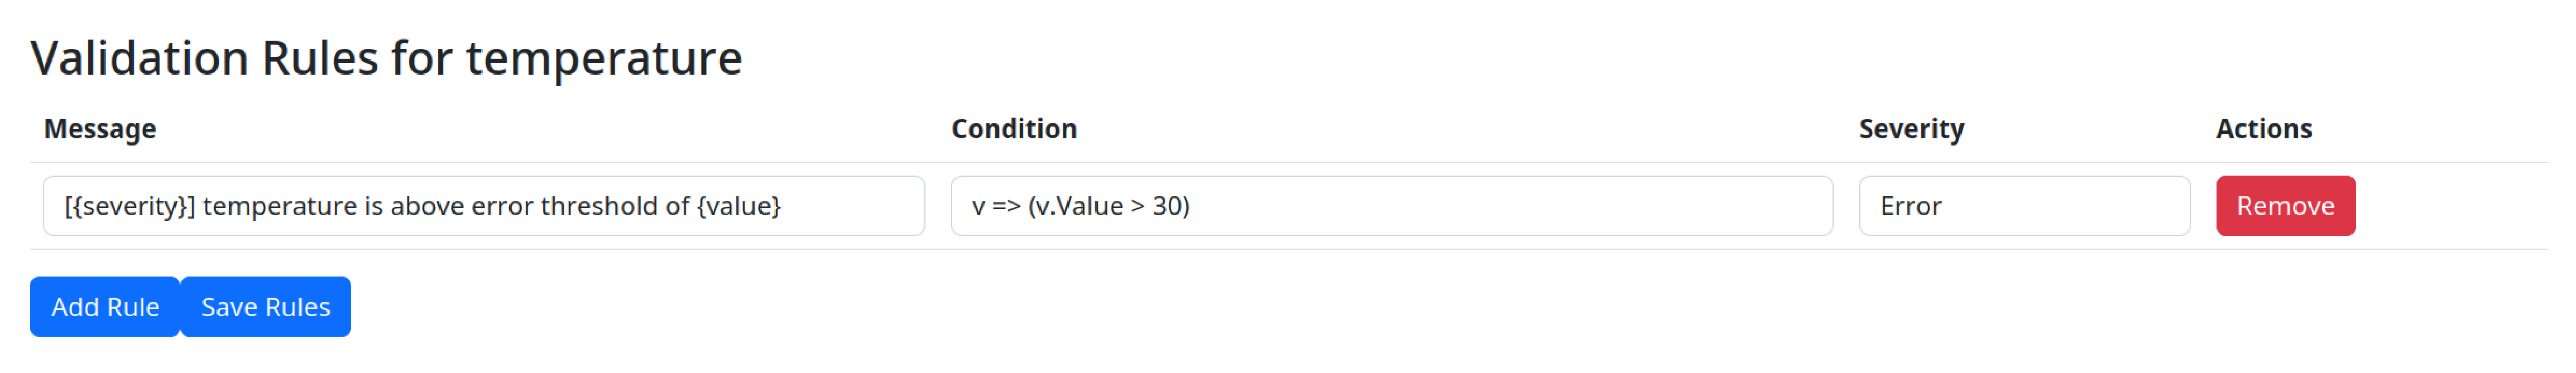
\includegraphics[width=\textwidth]{validation_rule}
  \caption{Przykładowa konfiguracja zasad walidacji}
  \label{atmosphere:validation_rule}
\end{figure}
Te reguły pozwalają na ustalenie dowolnej wiadomości opcjonalnie zawierającej referencje
do wartości odczytu (\textit{value}) oraz jego poziomu (\textit{severity}). Poziom może zostać
dostosowany przez użytkownika w zależności od priorytetu danej wiadomości.
Są one podzielone na trzy kategorie: informacje, ostrzeżenia oraz błędy.
Same reguły tworzone są za pomocą składni LINQ używanej w językach programowania
bazujących na środowisku .NET. Umożliwia to na konstrukcję bardziej zaawansowanych reguł
pozwalających na porównywanie wielu wartości, np. aplikacja może wysyłać powiadomienie, gdy
wartość odczytu przekroczy dany próg wyrażony w stopniach Celsjusza lub zupełnie inny
w stopnia Fahrenheita poprzez podanie dodatkowego porównania z polem jednostki (\textit{Unit}).
Przykład takiego wyrażenia przedstawiony został na Rys. \ref{atmosphere:custom_validation}.
\begin{figure}[h!]
  \centering
  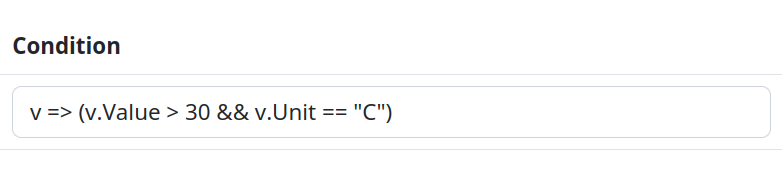
\includegraphics[width=\textwidth]{custom_validation}
  \caption{Przykładowa konfiguracja zasad walidacji ze specyfikacja jednostki}
  \label{atmosphere:custom_validation}
\end{figure}
Aplikacja umożliwia również konfigurację metody wysyłania powiadomień na adres email.
Administrator może skonfigurować takie parametry jak serwer SMTP oraz port wykorzystywany
do wysyłania wiadomości jak i nazwę użytkownika oraz hasło użyte do autoryzacji na nim.
Dodatkowo może on podać adres email, z którego dana wiadomość jest wysyłana jak i również
docelowy adres email. Przykładowa konfiguracja została zaprezentowana na Rys. \ref{atmosphere:email_configuration}.
\begin{figure}[h!]
  \centering
  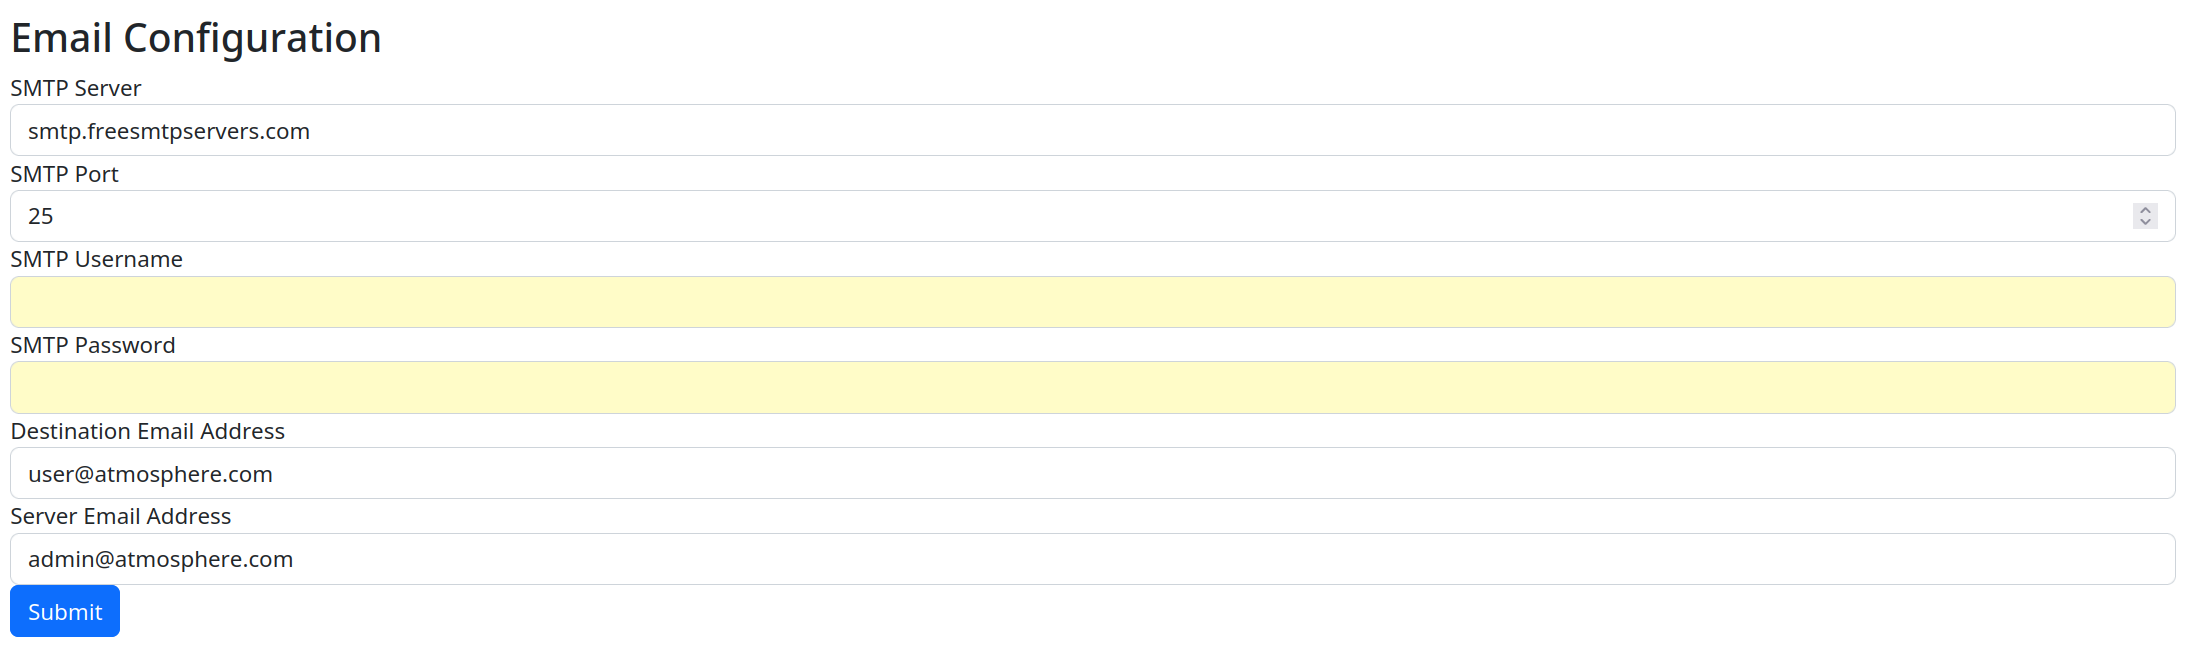
\includegraphics[width=\textwidth]{email_configuration}
  \caption{Przykładowa konfiguracja powiadomień email}
  \label{atmosphere:email_configuration}
\end{figure}

Po zalogowaniu na stronie głównej wyświetlane są wykresy przedstawiające zmianę danych odczytów w czasie.
Dane przedstawione są w postaci wykresu liniowego jako średnia odczytów w danej godzinie.
Ten widok został przedstawiony na Rys. \ref{atmosphere:charts}.
\begin{figure}[h!]
  \centering
  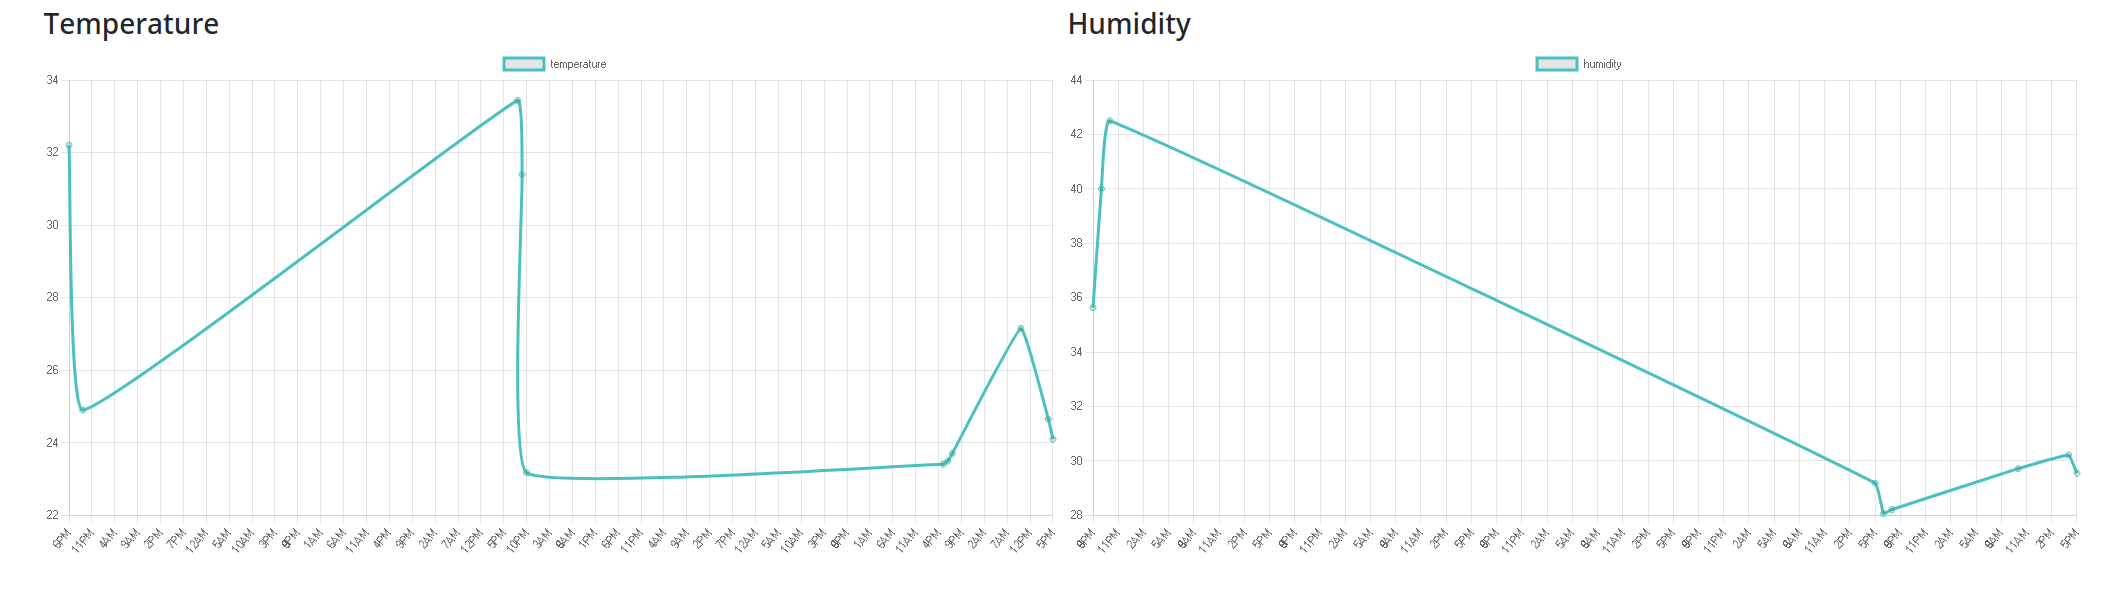
\includegraphics[width=\textwidth]{charts}
  \caption{Widok wykresów}
  \label{atmosphere:charts}
\end{figure}

Kolejnym widokiem jest lista odczytów parametrów środowiska. Użytkownik może 
filtrować ją z użyciem daty startowej i/lub daty końcowej po czym uzyskuje
wyniki znajdujące się w tym przedziale. Przykład przefiltrowanych danych
został przedstawiony na rysunku \ref{atmosphere:readings}.
\begin{figure}[h!]
  \centering
  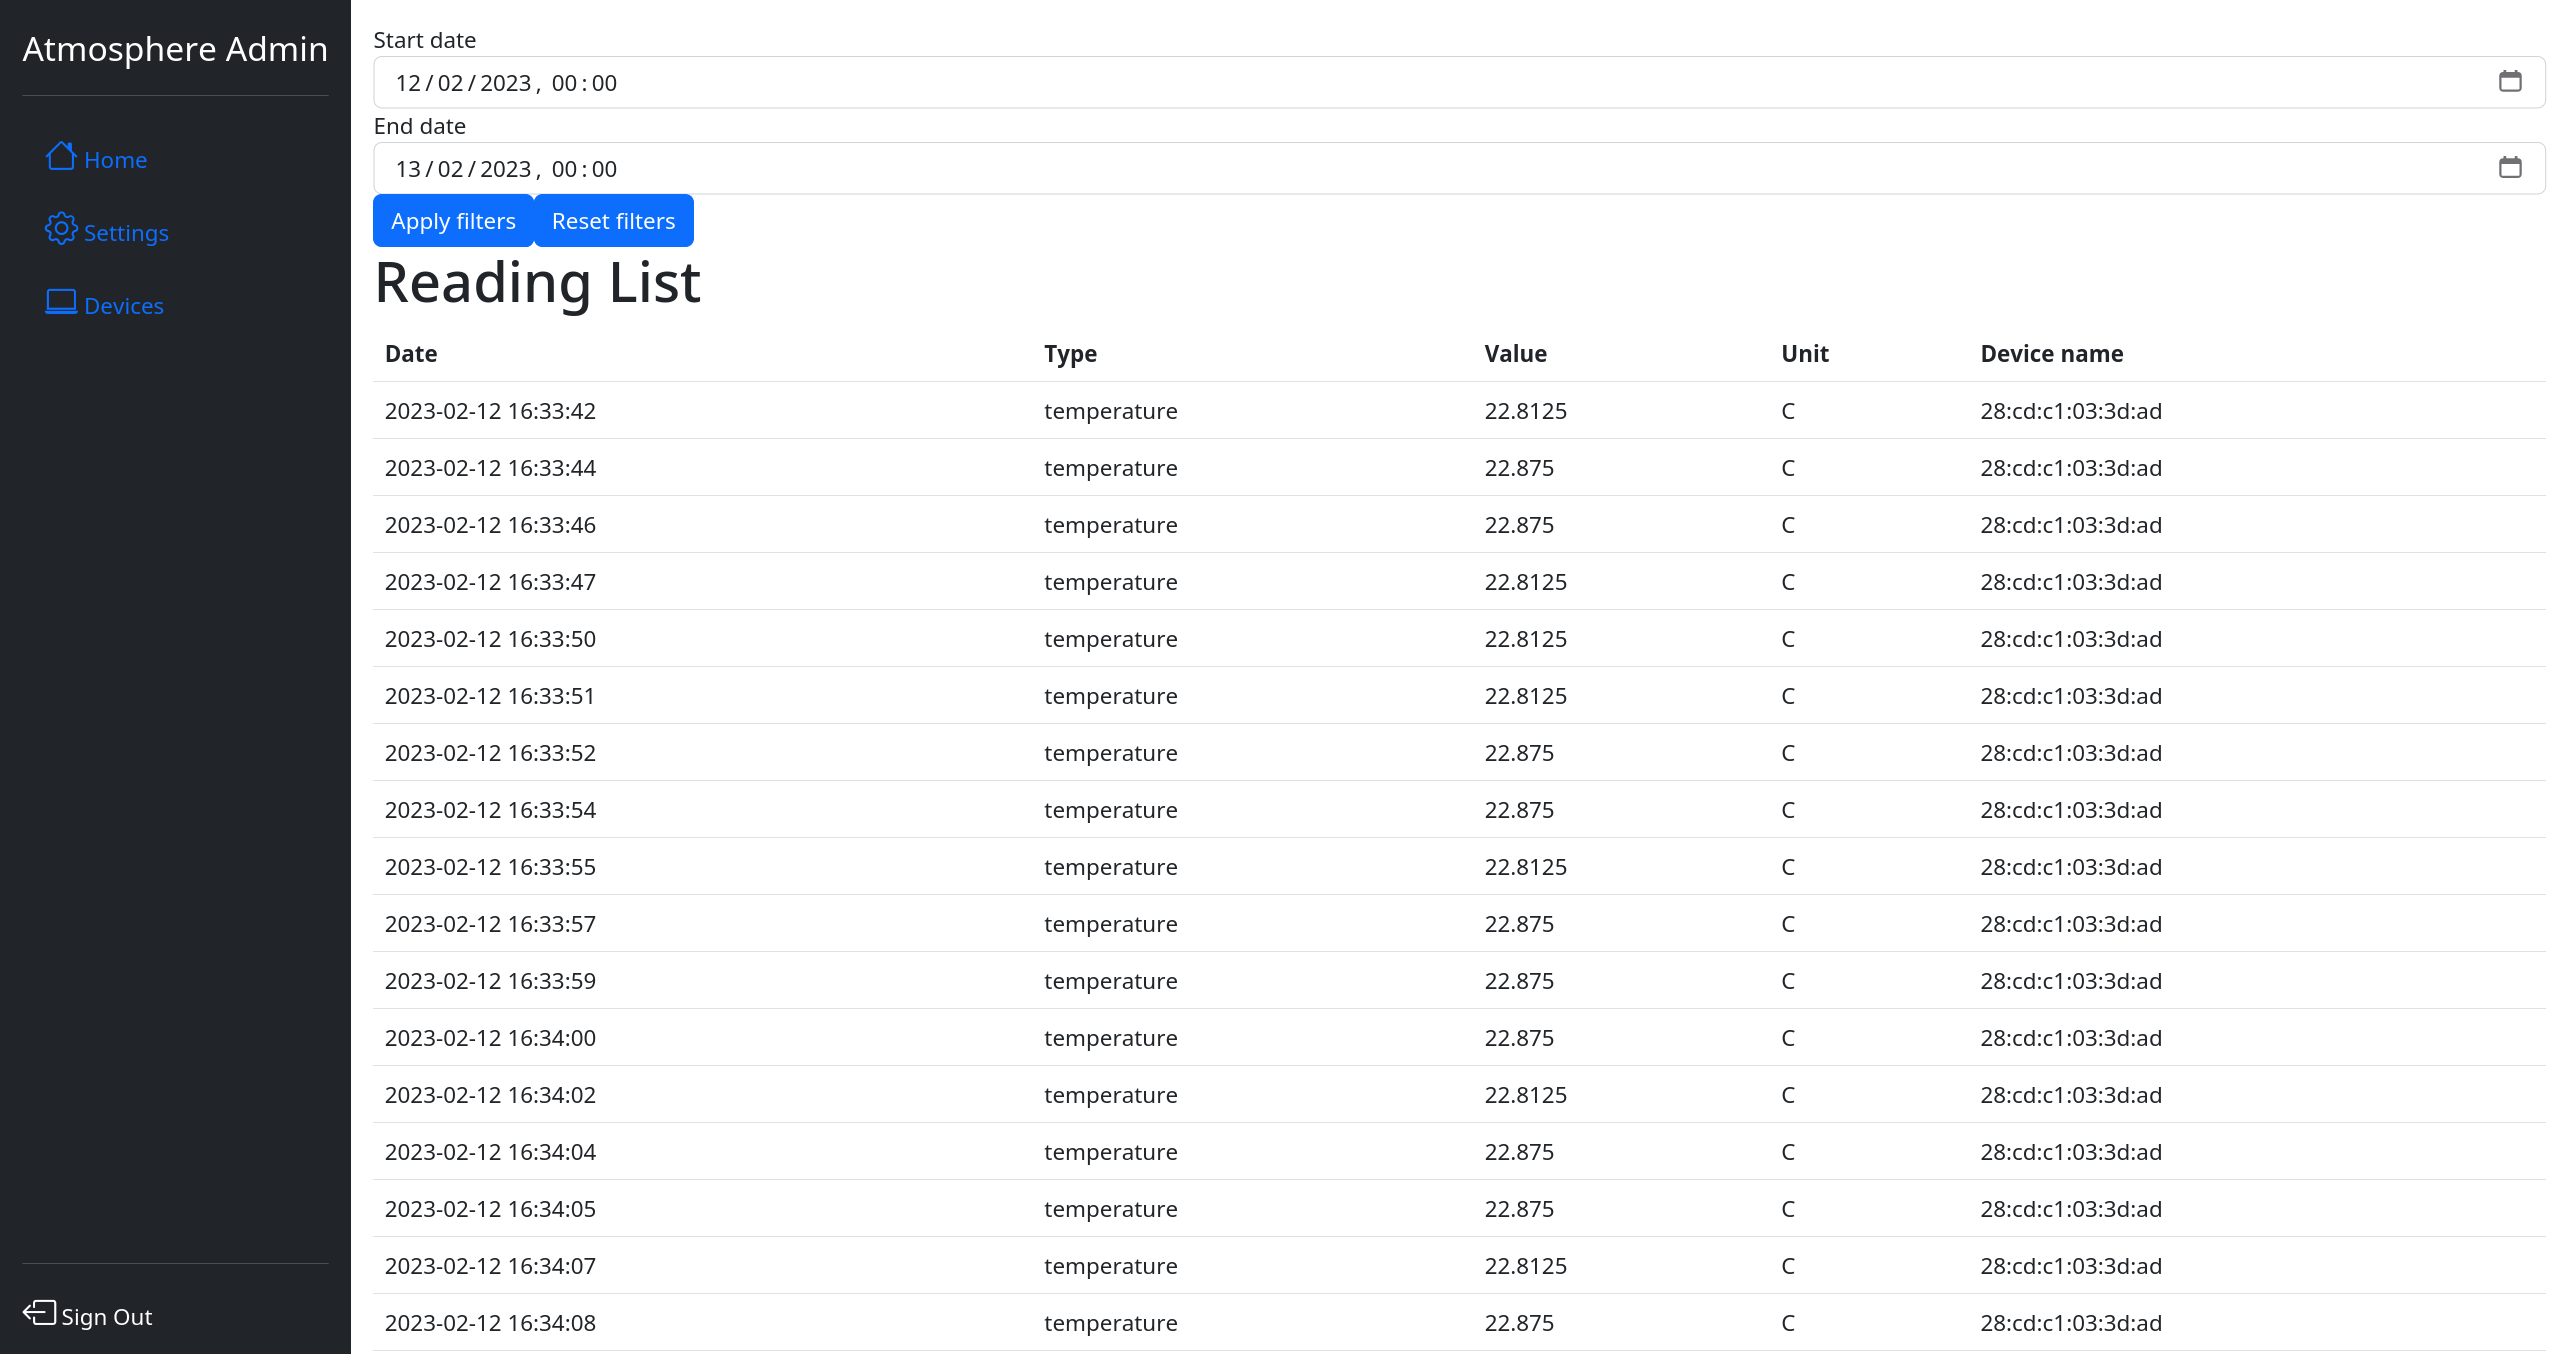
\includegraphics[width=\textwidth]{readings}
  \caption{Widok odczytów parametrów środowiska}
  \label{atmosphere:readings}
\end{figure}
Widok przedstawia w formie tabeli datę oraz czas wykonania odczytu, jego typ,
jednostkę pomiaru oraz adres fizyczny urządzenia pomiarowego.

Aplikacja posiada również widok urządzeń oraz ich stanu. Umożliwia on administratorowi
na aktywację bądź dezaktywację danego urządzenia oraz posiada informacje o tym czy 
dane urządzenie jest aktualnie połączone z systemem.
Ten widok został przedstawiony na Rys. \ref{device_list}.
\begin{figure}[h!]
  \centering
  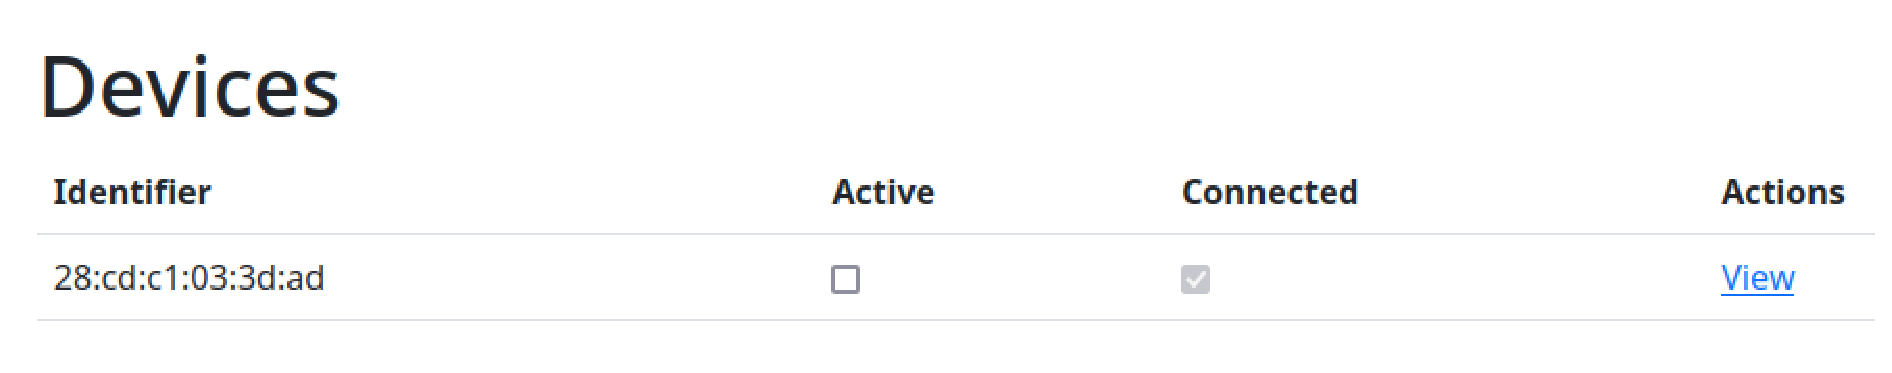
\includegraphics[width=\textwidth]{connect_dev}
  \caption{Urządzenie na liście urządzeń}
  \label{device_list}
\end{figure}
Aplikacja pozwala na przeglądanie odczytów wykonanych przez dane urządzenie, podgląd wykresów
stworzonych z danych urządzenia oraz ustawień specyficznych dla urządzenia tj. reguły walidacji
oraz czas między wykonywaniem pomiarów. Dwa pierwsze nie różnią się widokiem od standardowych 
komponentów poza przefiltrowanymi danymi, natomiast ustawienia urządzenia przedstawiono na 
rys. \ref{atmosphere:device_settings}.
\begin{figure}[h!]
  \centering
  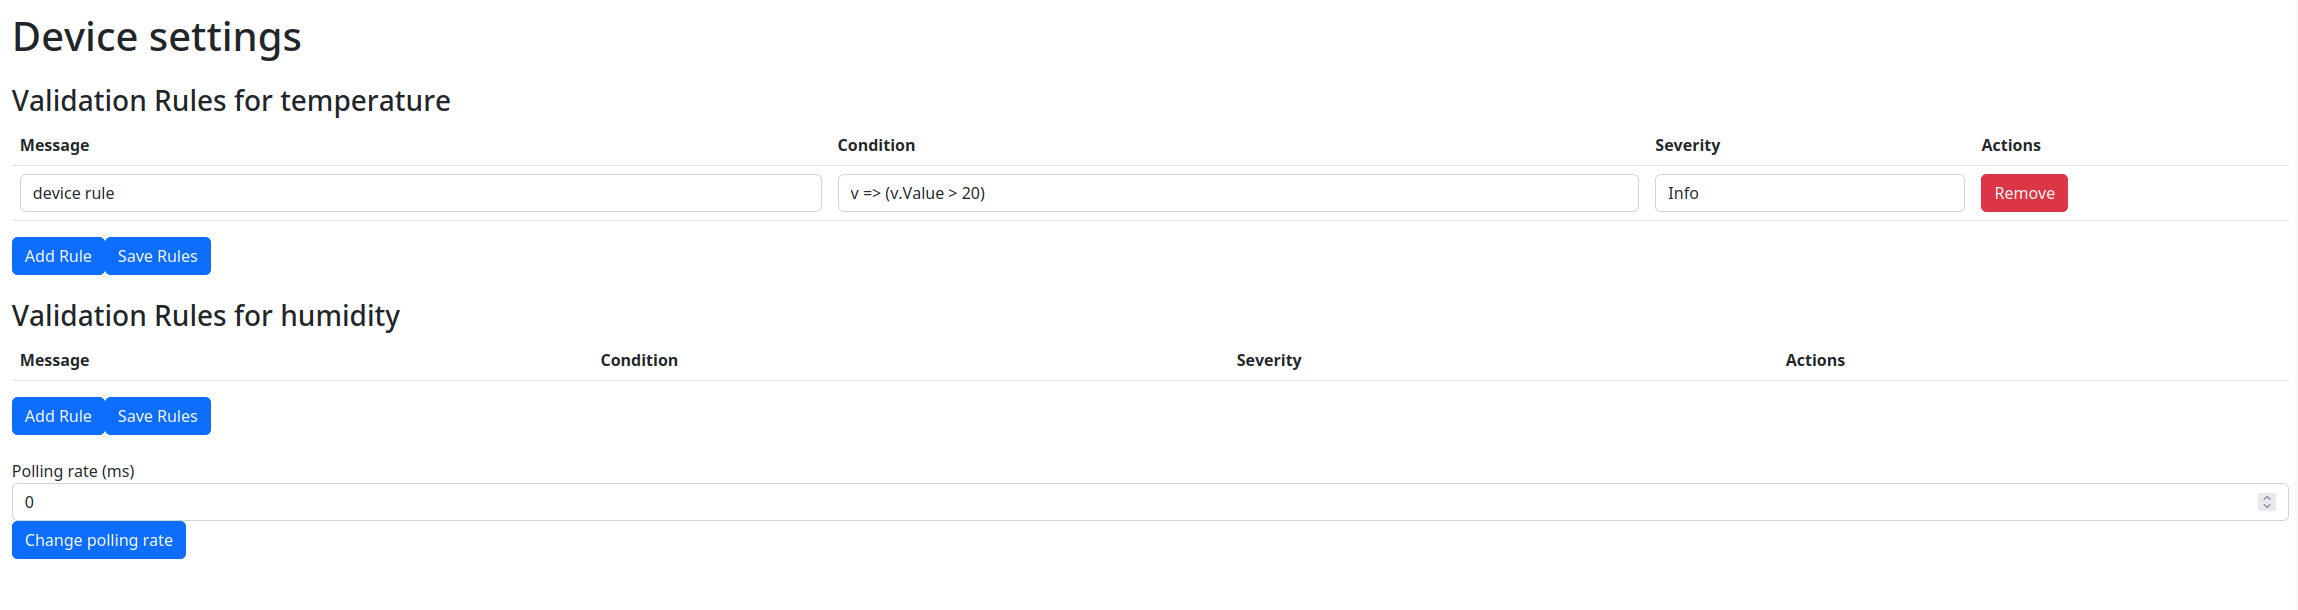
\includegraphics[width=\textwidth]{device_settings}
  \caption{Ustawienia urządzenia}
  \label{atmosphere:device_settings}
\end{figure}

Ostatnim widokiem jest widok listy użytkowników. Pozwala ona administratorowi na tworzenie
nowych kont użytkowników oraz ich usuwanie. Lista użytkowników została przedstawiona
na Rys. \ref{users}, a formularz służący do ich tworzenia na Rys. \ref{create_user}.
\begin{figure}[h!]
  \centering
  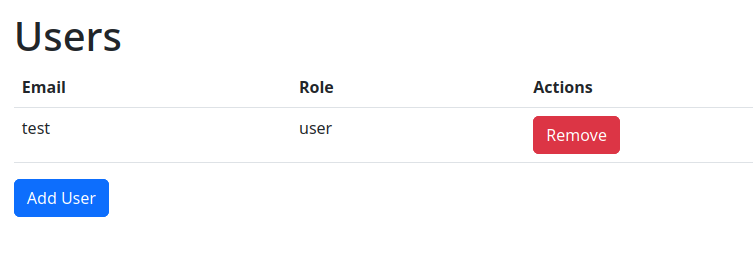
\includegraphics[width=\textwidth]{users}
  \caption{Lista użytkowników}
  \label{users}
\end{figure}
\begin{figure}[h!]
  \centering
  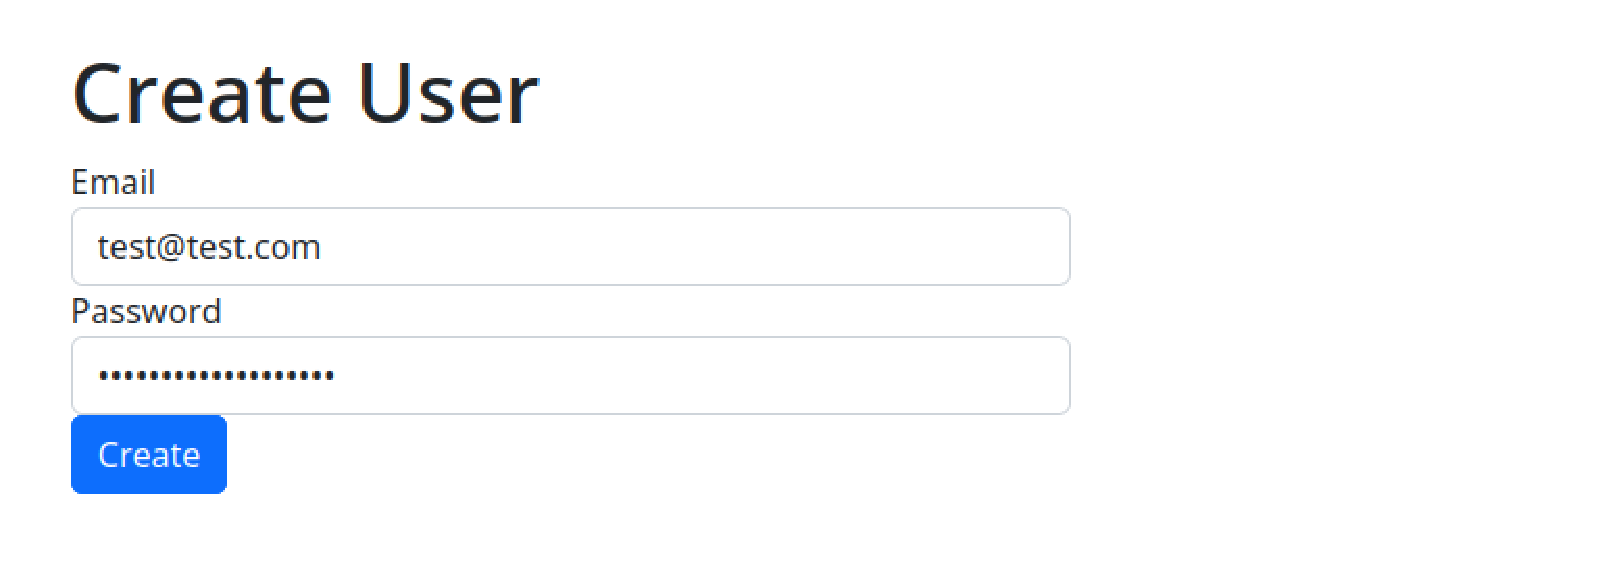
\includegraphics[width=\textwidth]{create_user}
  \caption{Formularz tworzenia użytkowników}
  \label{create_user}
\end{figure}
